\documentclass[kravspec/krav.tex]{subfiles}

\begin{document}

\section{Översikt av systemet}

\begin{figure}[h]
    \centering
    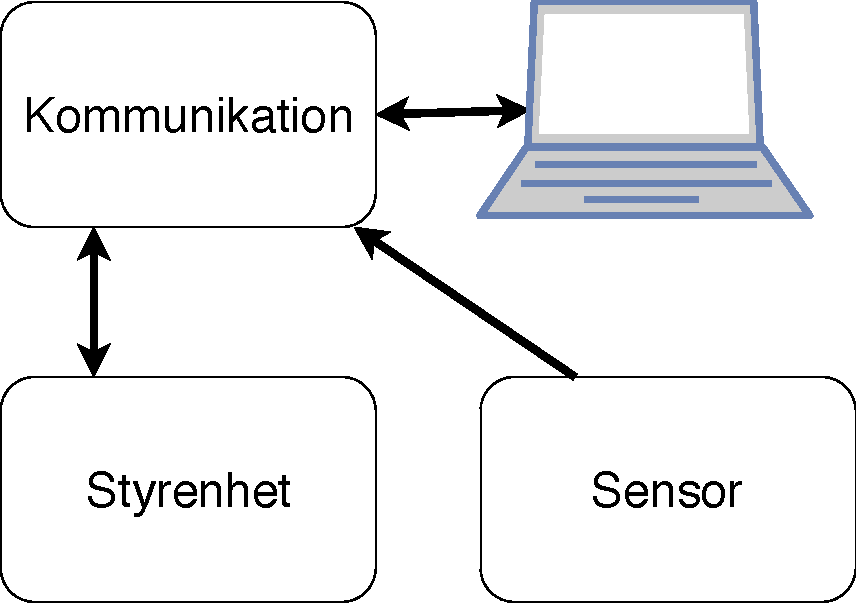
\includegraphics[width=0.6\linewidth]{kravspec/figures/overview-schema.pdf}
    \caption{Grov blockschema över moduler i produkten}
    \label{fig:overview}
\end{figure}

\subsection{Grov beskrivning av produkten}
Produkten är en bil med fyra hjul som ska med hjälp av ett känt vägnät ta sig
till en passagerare och skjutsa passageraren till önskad destination. Denna
taxibil ska kunna åka framåt, bakåt, svänga vänster och höger.  Bland annat ska
man kunna initiera en bblåtandslänk mellan bilen och en dator som har stöd för
blåtand. Bilen ska ha ett läge där man kan fjärrstyra bilen och ett läge där
bilen ska köra autonomt i vägnätet samt undvika hinder.

\subsection{Produktkomponenter}
Lämplig hårdvara med kompletterande mjukvara kommer finnas i den kompletta
produkten.  Bland annat ska även tekniskt dokumenation ingå i produkten.

\subsection{Beroenden till andra system}
Fjärstyrning av bilen skall vara beroende av en dator som har stöd för blåtand.
Autonoma läget aktiveras från användargränsnittet tillgänglig på datorn med
blåtand.

\subsection{Ingående delsystem}
En kommunikationsenhet, en styrmodul och en sensormodul enligt figur
\ref{fig:overview}. Sensormodulen ska hämta in data om omgivningen, bland annat
ska vi ha en kamera som tar bilder av vad som är framifrån, en sensor som mäter
avstånd till objekt i omgivning och tejpföljare som sensorer. Lämplig data av
omgivning skickas till kommunikationsmodell. Produkten har även en styrmodul
som ser till att bilen kan styras beroende på data från kommunikationsmodul.

\subsection{Avgränsningar}
Vi tar inte hänsyn till små väghinder som grova vägkanter och gropar.  Vi utgår
ifrån att vägen består av hinder som är i lämplig höjd för våra sensorer att
upptäcka. Med andra ord, vi antar att vägen är jämn och fin där eventuella
gropar inte finns.

\end{document}
